\documentclass[handout]{beamer}
\usefonttheme{professionalfonts}
\RequirePackage{thesis-slides}

\setbeameroption{show notes on second screen=bottom}

\begin{document}
\hspace*{-1.2cm}
\begin{frame}[plain]
\titlepage % Print the title page as the first slide
\end{frame}

\begin{frame}
  \frametitle{Supervised Learning}
  Our idea is to build a theoretical setting that incorporates all the features real model,
  but at the same time, it's modelized enough to be studied theoretically.
\end{frame}

\section{The model}
\begin{frame}
\frametitle{The model: architecture}
Goal: learn a \emph{predictor} \(\hat{f}\) given some samples \((\vec{x},y)\in\Real^{d+1}\).
\vfill
\begin{columns}
  \column{0.4\textwidth}
    \structure{Soft Committee Machine}
    \vspace{1.5pt}

    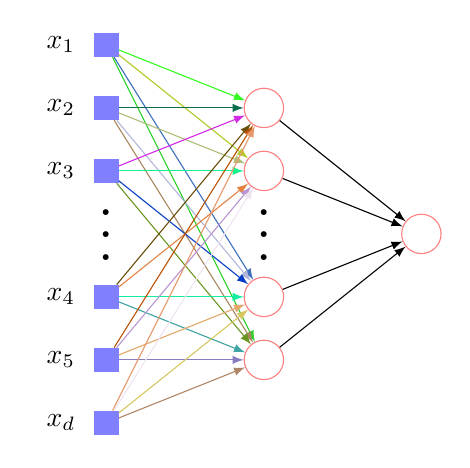
\begin{tikzpicture}[x=1cm, y=.8cm, >=latex]
      \tikzset{
  inputnode/.style={
    rectangle,
    draw,
    minimum size=.3cm
  },
  every neuron/.style={
    circle,
    draw,
    minimum size=.5cm
  },
  neuron missing/.style={
    draw=none, 
    fill=none, %<- added
    scale=2,
    text height=0.333cm,
    execute at begin node=\color{black}$\vdots$
  }
}

\pgfmathparse{rnd}
\xdefinecolor{MyColor}{rgb}{\pgfmathresult, 1.0, 1.0}

\foreach \m [count=\y] in {1,2,3,missing,4,5,6} %<- removed "/\l" here 
  \node [fill=black,inputnode/.try, neuron \m/.try,blue!50] (input-\m) at (0,2.5-\y) {};
% added "fill=green" in the line above

\foreach \m [count=\y] in {1,2,missing,3,4}
  \node [every neuron/.try, neuron \m/.try,red!50] (hidden-\m) at (2,1.5-\y) {};

\foreach \m [count=\y] in {1}
  \node [every neuron/.try, neuron \m/.try,red!50] (output-\m) at (4,-.5-\y) {};

\foreach \l [count=\i] in {1,2,3,4,5,d}
  \path (input-\i) -- ++(-1,0)
   node [midway] {$x_\l$};

% \foreach \l [count=\i] in {1,n}
%   \draw [->] (output-\i) -- ++(1,0)
%    node [above, midway] {$a_\l$};

\foreach \i in {1,...,6}
  \foreach \j in {1,...,4} {
    \edef\R{\pdfuniformdeviate 255}
    \edef\G{\pdfuniformdeviate 255}
    \edef\B{\pdfuniformdeviate 255}
    \xdefinecolor{MyColor}{RGB}{\R,\G,\B}
    \draw [->,MyColor] (input-\i) -- (hidden-\j);
  }


\foreach \i in {1,...,4}
  \foreach \j in {1}
    \draw [->] (hidden-\i) -- (output-\j);

% \foreach \l [count=\x from 0] in {Eingangs-, Ausgangs-}
%   \node [align=center, above] at (\x*4,2) {\l \\ Neuronen};
    \end{tikzpicture}
  \column{0.6\textwidth}
    \[\hat{f}\colon \Real^d\to\Real\]
    \[\hat{f}{(\vec{x})} = \frac{1}{p}\sum_{j=1}^{p} \act{\left(\frac{\vec{w}_j \cdot \vec{x}}{\sqrt{d}}\right)}\]
    \vspace{30pt}

    \begin{center}The network \emph{parameters} are\end{center} 
    \[\vec{w}_j \coloneqq [\W]_j \in \Real^d\]
    \[\W \in \Real^p\times\Real^d\]
\end{columns}
\note[item]{Must define \(d, p, \act\). They are \textbf{meta}parameters}
\note[item]{Stress the fact that the \emph{hat} is for the predictor.}
\note[item]{Just one real output, but it's not a problem.}
\note[item]{Fixed weights in the second layer, can be done with more but it's just complicated.
            More parameters, no gain.}
\end{frame}

\begin{frame}
  \frametitle{The model: data samples}
  \(\vec{x}\) samples are \emph{indipendent normal distributions}
  \[
    \vec{x} \sim \gauss{(0,\I_d)}.
  \]
  \pause

  The \(y\) is generated by a \emph{teacher} model with the same architecture
  \[
    f{(\vec{x})} = \frac{1}{k}\sum_{r=1}^{k} \act{\left(\frac{\vec{w}^*_r \cdot \vec{x}}{\sqrt{d}}\right)}
    \quad\text{where}\quad \vec{w}^*_r \coloneqq [\W^*]_r \in \Real^d. 
  \]
  \pause

  We overlap some noise to the \(y\) label
  \[
    y = f{(\vec{x}) + \sqrt{\Delta}\xi}\quad\text{with } \xi \sim \gauss{(0,1)}
  \]
  \note[item]{
    We use Gaussians, but it's not mandatory. It has been done in the past \cite{refinetti2022dynamics}
  }
  \note[item]{
    \emph{Teacher-student setting}: the student knows anything about the architecture of the teacher.
    He observes only pairs. It's just a convenient way of writing a generative model that gives us control on the learning.
  }
  \note[item]{
    The teacher has \(k\le p\) as a realizability condition
  }
  \note[item]{
    Teacher has not the hat and the weights matrix has the asterisk
  }
  \note[item]{
    Must say \(\Delta\) is not a parameter of the network, but just a parameter of our theoretical model.
  }
\end{frame}

\begin{frame}
  \frametitle{The model: measuring the goodness}
  The \emph{loss function} measures distance in output spaces
  \[
    \only<1>{\loss\colon \Real\times\Real\to\Real^+}
    \only<2->{\loss\colon \Real\times\Real\to\Real^+ \qquad \loss{(y_1,y_2)}=\frac12 (y_1-y_2)^2}
  \]
  \pause

  The goodness of the \emph{predictor} over a sample \((\vec{x}_s,y_s)\) is 
  \[
    \loss{\left(\hat{f}{(\vec{x}_s)},y_s\right)}
  \]
  \pause

  The global performance instead
  \[
    \risk_\text{theo} 
    %= \E_{\vec{x}\sim\gauss{(0,\I_d)}}{\left[\loss{\left(f{\left(\vec{x}\right)},\hat{f}{\left(\vec{x}\right)}\right)}\right]}=
    =\frac{1}{2}\E_{\vec{x}\sim\gauss{(0,\I_d)}}{\left[\left(f{\left(\vec{x}\right)}-\hat{f}{\left(\vec{x}\right)}\right)^2\right]}
  \]
  \note[item]{
    The loss function is an important choice and really depends on the data used.
    Since we are working in a continuous setting this is the easiest choice.
    Moreover, it will lead to known models in the future (phase retrieval)
  }
  \note[item]{
    We have access to the theoretical risk just because we know both the distribution of \(\vec{x}\) and the
    generative model (teacher). We don't use it for the training, otherwise, we are not studying the realistic dynamics.
  }
  \note[item]{
    The risk is called theoretical because there is also the empirical one, on the sample one really knows, but it's not the case here.
  }
\end{frame}

\begin{frame}
  \frametitle{The model: the algorithm}
  \begin{block}{Optimization}
    The best possible predictor has parameters
    \[
      \W_\text{best} \in \argmin_{\W}{\risk_\text{theo}}
    \]
  \end{block}
  \pause

  The algorithm we use is \emph{one-pass stochastic gradient descent}:
  \begin{enumerate}
    \item Sample a vector \(\vec{x}^\nu\) and generate \(y^\nu\) using the teacher.
    \item For every \(j\in[1,p]\)
          \[\w^{\nu+1}_j = \w^{\nu}_j - \gamma \nabla_{\w_j}\left(\loss\left(y^\nu,\hat{f}{\left(\vec{x}^\nu\right)}\right)\right)\]
  \end{enumerate}
  \pause

  \vspace{-15pt}
  \begin{alertblock}{Open question}
    The loss function is not convex, but the algorithm converges to nearly optimal solution
  \end{alertblock}

  \note[item]{
    Of course, the \(\argmin\) is not unique, but it's not important!
  }
  \note[item]{
    \(\nu\) is the index that indicates the number of samples used.
  }
  \note[item]{
    The formula is the update rule of the weights.
  }
  \note[item]{
    \(\gamma\) is the \emph{learning rate}. It's an \textbf{hyper}parameter, a property only of the algorithm. 
    It affects the dynamics and the final state, but it's not something that the predictor knows.
  }
  \note[item]{
    If someone among you has experience in applying machine learning maybe it's used to \emph{full batch gradient descent} or
    \emph{stochastic gradient descent}, but also this algorithm is use.
  }
  \note[item]{
    Let's note that the training dynamics it's a discrete stochastic process in the space of the student weights matrix.
  }
\end{frame}

\section{High dimensional limit}
\begin{frame}
  \frametitle{Local fields}
  \begin{block}{Goal}
    Describe the training dynamic with some \emph{sufficient statics} of the weights
  \end{block}
  \pause
  \vfill

  \begin{columns}
    \column{0.5\textwidth}
      \structure{Change of variables}
      \includegraphics[width=\textwidth]{example-image-duck}
    \column{0.5\textwidth}
    \[
      \vec{\lf} = \frac{\W\vec{x}}{\sqrt{{d}}}\quad
      \vec{\lf}^{*} = \frac{\W^{*}\vec{x}}{\sqrt{{d}}}
    \]
    \[\begin{split}
        \hat{f}{(\vec{x})} \rightarrow& \hat{f}{(\vec{\lf})} = \frac{1}{p}\sum_{j=1}^{p} \act{\left(\lf_j\right)} \\
        f{(\vec{x})} \rightarrow& f{(\vec{\lf}^*)} = \frac{1}{k}\sum_{r=1}^{k} \act{\left(\lf^*_k\right)}
    \end{split}\]

  \end{columns}
  \note[item]{
    I want to do all the steps of this derivation (no calculations) to emphatize how this is 
  }
  \note[item]{
    The \(\lf\)s are called \emph{local fields} and are microscopic variables.
    They are correlated normal distributions, their scale is around 1 independently of \(d\). We see this in the next slides
  }
\end{frame}

\begin{frame}
  \frametitle{Order parameters}
  \(\vec{\lf},\vec{\lf}^*\) are normal random variables with 0 mean and covariance
  \[
    \frac{1}{d}\left(\begin{array}{cc}\W\W^\top &  \W\W^{*\top}\\ \W^{*}\W^\top & \W^*\W^{*\top}\end{array}\right) =
    \left(\begin{array}{cc}\Q & \M \\ \M^{\top} & \P \end{array}\right) =
    \vec{\Omega} \in \Real^{p+k}\times\Real^{p+k}
  \]
  \(\vec{\Omega}\) is the \emph{overlapping matrices};\\
  \(\Q,\M,\P\) are the \emph{order parameters}
  \pause 

  \vfill
  \(\vec{\Omega}\) is the sufficient statistic we use for describing the process
  \[
    \risk_\text{theo}= \frac12\E_{\vec{\lf},\vec{\lf^* \sim \gauss{(0,\vec{\Omega})}}}
                              {\left[\left(f{(\vec{\lf}^*)} - f{(\vec{\lf})}\right)^2\right]} = \risk{(\vec{\Omega})}
  \]
  \note[item]{
    The variance allows us to define the \emph{order parameters}. These are the \emph{macroscopic variable} of the system
    because they are not dependent on \(d\) order of magnitude.
  }
  \note[item]{
    They are sufficient statics because \(\Omega\) is enough for defining the distribution of the local fields.
  }
\end{frame}

\begin{frame}[fragile]
  \frametitle{Update rule for order parameters}
  \[
    \left[\M^{\nu+1}\right]_{jr} = \frac{\w^{\nu+1}_j \w^{*\top}_r}{d}
    = \cdots = \left[\M^{\nu}\right]_{jr} + \frac{1}{d} \psi_{jr}{(\vec{\lf}^\nu,\vec{\lf}^{*\nu})}
  \]
  \pause
  \[
    \left[\Q^{\nu+1}\right]_{jl} 
    = \left[\Q^{\nu}\right]_{jl} + \frac{1}{d}\varphi_{jl}{(\vec{\lf}^\nu,\vec{\lf}^{*\nu})}
    \qquad \P\text{ is constant}
  \]
  \pause

  \begin{block}{Overlapping matrix dynamic}
    \[\left\{\vec{\Omega}^\nu \in \Real^{(p+k)\times(p+k)}|\nu\in\Natural\right\}\]
    \[
      \begin{tikzcd}
      \vec{\Omega}^0 \arrow[r,"\text{sample}"] \arrow[d] & \vec{\lf}^1,\vec{\lf}^{*1} \arrow[r,"\text{update}"] & \vec{\Omega}^1 \arrow[d] \arrow[r,dash,dotted] & \vec{\lf}^\nu,\vec{\lf}^{*\nu} \arrow[r,"\text{update}"] & \vec{\Omega}^\nu \arrow[d]\\
      \risk^0 & {} & \risk^1 & {} & \risk^\nu
      \end{tikzcd}
    \]
  \end{block}

  \note[item]{
    We can use the update rule on weights to compute an update rule on parameters.
    It's not obvious that it's possible to have an update rule on order parameters, but we did.
  }
  \note[item]{
    We can fully describe the learning process by looking at the dynamic of matrix \(\vec{\Omega}\).
    The risk is just a function of \(\Omega\), so there is no need to keep all the weights to monitor learning (we gain a lot in term of storage of information).
    Nevertheless, we will use the weights matrix properties in simulations or for initialization, but the theoretical study can be restricted to this matrix!
  }
\end{frame}

\begin{frame}
  \frametitle{High dimensional limit}
  We take the limit \(d\to+\infty\)
  \[
    \frac{\M^{\nu+1} - \M^{\nu}}{\frac1d} = \vec{\psi}{(\vec{\lf}^\nu,\vec{\lf}^{*\nu})}
    \qquad \delta t = \frac1d 
  \]
  \pause

  \begin{exampleblock}{Differential Equations of the process}
    \begin{align*}
      \dod{\M{\left(t\right)}}{t} &=\E_{\vec{\lf},\vec{\lf^* \sim \gauss{(0,\vec{\Omega}{(t)})}}}{\left[\psi{(\vec{\lf}^\nu,\vec{\lf}^{*\nu})}\right]} \eqqcolon \Psi{\left(\vec{\Omega}\right)}\\
      \dod{\Q{\left(t\right)}}{t} &=\E_{\vec{\lf},\vec{\lf^* \sim \gauss{(0,\vec{\Omega}{(t)})}}}{\left[\phi{(\vec{\lf}^\nu,\vec{\lf}^{*\nu})}\right]} \eqqcolon \Phi{\left(\vec{\Omega}\right)},
    \end{align*}
    \vspace{-10pt}
    \begin{itemize}
      \item Discrete index is mapped to time with \(t=\frac{\nu}{d}\)
      \item The expected error between the two is given by \(\frac{1}{\sqrt{d}}\)
    \end{itemize}
  \end{exampleblock}

  \note[item]{
    LHS is the derivative of the order parameter matrix;
    RHS is less clear. The intuition is given by the CLT: the fluctuations are killed beacuse we are using a lot of indipendent gaussian.
    RHS concentrates to the mean and converges to the expected value of the expression.
    Again this depends only on the shape of the distribution of \(\lf\)s, so this expected value is function of just \(\vec{\Omega}\)
  }
  \note[item]{
    The differential equations depend on \(\gamma, p, k, \sigma\)
  }
  \note[item]{
    These equations are the fundamental result used in this work relay on.
    They give us a \emph{deterministic} dynamic for the evolution, starting from a stochastic process
  }
  \note[item]{
    There is a formal formulation of this fact given by \cite{goldt2019dynamics}. It's mathematically proved! 
  }
\end{frame}


\setbeamertemplate{page number in head/foot}{\phantom{0/0}}
\begin{frame}[noframenumbering, allowframebreaks]
  \frametitle{Bibliography}
  % \textbf{\structure{Bibliography}}
  \printbibliography
  \vspace{3cm}
\end{frame}

\begin{frame}{}
  \frametitle{}
\end{frame}

\end{document}
